% This file was created with tikzplotlib v0.10.1.
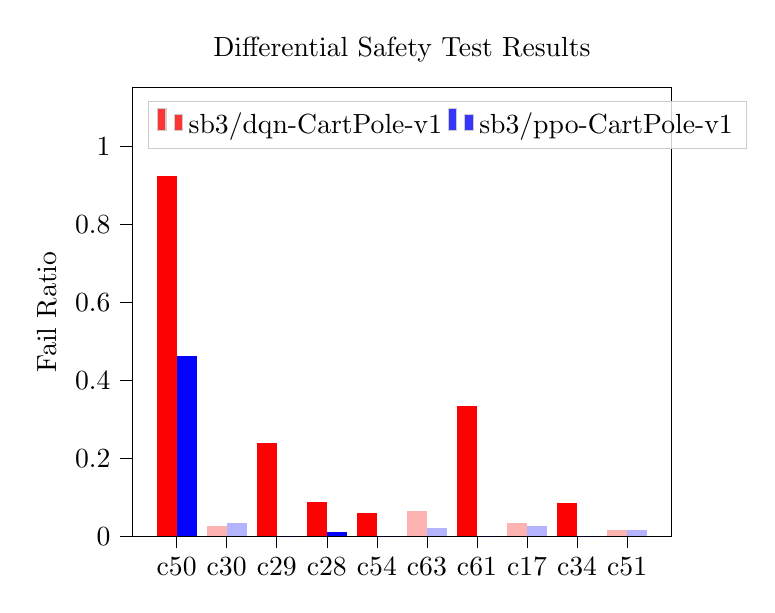
\begin{tikzpicture}

\definecolor{blue33252}{RGB}{3,3,252}
\definecolor{darkgray176}{RGB}{176,176,176}
\definecolor{lightgray204}{RGB}{204,204,204}
\definecolor{red25233}{RGB}{252,3,3}

\begin{axis}[
legend cell align={left},
legend columns=3,
legend style={
  fill opacity=0.8,
  draw opacity=1,
  text opacity=1,
  at={(0.03,0.97)},
  anchor=north west,
  draw=lightgray204
},
tick align=outside,
tick pos=left,
title={Differential Safety Test Results},
x grid style={darkgray176},
xmin=-0.49, xmax=10.29,
xtick style={color=black},
xtick={0.4,1.4,2.4,3.4,4.4,5.4,6.4,7.4,8.4,9.4},
xticklabels={c50,c30,c29,c28,c54,c63,c61,c17,c34,c51},
y grid style={darkgray176},
ylabel={Fail Ratio},
ymin=0, ymax=1.15,
ytick style={color=black}
]
\draw[draw=none,fill=red25233] (axis cs:-2.77555756156289e-17,0) rectangle (axis cs:0.4,0.923076923076923);
\addlegendimage{ybar,ybar legend,draw=none,fill=red25233}
\addlegendentry{sb3/dqn-CartPole-v1}

\draw[draw=none,fill=red25233] (axis cs:2,0) rectangle (axis cs:2.4,0.238095238095238);
\draw[draw=none,fill=red25233] (axis cs:3,0) rectangle (axis cs:3.4,0.0888888888888889);
\draw[draw=none,fill=red25233] (axis cs:4,0) rectangle (axis cs:4.4,0.0588235294117647);
\draw[draw=none,fill=red25233] (axis cs:6,0) rectangle (axis cs:6.4,0.333333333333333);
\draw[draw=none,fill=red25233] (axis cs:8,0) rectangle (axis cs:8.4,0.0857142857142857);
\draw[draw=none,fill=blue33252] (axis cs:0.4,0) rectangle (axis cs:0.8,0.461538461538462);
\addlegendimage{ybar,ybar legend,draw=none,fill=blue33252}
\addlegendentry{sb3/ppo-CartPole-v1}

\draw[draw=none,fill=blue33252] (axis cs:2.4,0) rectangle (axis cs:2.8,0);
\draw[draw=none,fill=blue33252] (axis cs:3.4,0) rectangle (axis cs:3.8,0.0111111111111111);
\draw[draw=none,fill=blue33252] (axis cs:4.4,0) rectangle (axis cs:4.8,0);
\draw[draw=none,fill=blue33252] (axis cs:6.4,0) rectangle (axis cs:6.8,0);
\draw[draw=none,fill=blue33252] (axis cs:8.4,0) rectangle (axis cs:8.8,0);
\draw[draw=none,fill=red25233,fill opacity=0.3] (axis cs:1,0) rectangle (axis cs:1.4,0.025);
\draw[draw=none,fill=red25233,fill opacity=0.3] (axis cs:5,0) rectangle (axis cs:5.4,0.065);
\draw[draw=none,fill=red25233,fill opacity=0.3] (axis cs:7,0) rectangle (axis cs:7.4,0.035);
\draw[draw=none,fill=red25233,fill opacity=0.3] (axis cs:9,0) rectangle (axis cs:9.4,0.015);
\draw[draw=none,fill=blue33252,fill opacity=0.3] (axis cs:1.4,0) rectangle (axis cs:1.8,0.035);
\draw[draw=none,fill=blue33252,fill opacity=0.3] (axis cs:5.4,0) rectangle (axis cs:5.8,0.02);
\draw[draw=none,fill=blue33252,fill opacity=0.3] (axis cs:7.4,0) rectangle (axis cs:7.8,0.025);
\draw[draw=none,fill=blue33252,fill opacity=0.3] (axis cs:9.4,0) rectangle (axis cs:9.8,0.015);
\end{axis}

\end{tikzpicture}
